\documentclass[conference]{IEEEtran}
\usepackage{graphicx}
\usepackage{amsmath}
\usepackage{cite}
\usepackage{subcaption} % For subfigures and captions
\usepackage{caption}
\captionsetup[figure]{labelformat=simple, labelsep=period}


\title{Waypoint Generation based on Crop Row Detection Using Aerial Imaging Systems}

\author{
	\IEEEauthorblockN{Alireza Amiri}
	\IEEEauthorblockA{Department of Electrical Engineering\\
		K N. Toosi University of Technology\\
		Tehran, Iran\\
		ali.amiri@email.kntu.ac.ir}
	\and
	\IEEEauthorblockN{Saeed Khankalantary}
	\IEEEauthorblockA{Department of Electrical Engineering\\
		K N. Toosi University of Technology\\
		Tehran, Iran\\
		s.kalantary@kntu.ac.ir}
}

\begin{document}
	
	\maketitle
	
	\begin{abstract}
		In autonomous agriculture, using wheeled mobile robots for various tasks requires the precise generation of waypoints to accurately define the robots' paths. This article presents a method that utilizes aerial imagery to detect crop positions and establish waypoints. A specialized hardware setup comprising a high-resolution camera, wireless transmitter, and receiver has been developed to capture and transmit live images of the agricultural field. In the image processing stage, crops are identified using two parallel techniques—Unet and K-means clustering. Subsequently, the integration of linear regression and Hough Transform is examined to detect crop row lines, refined through filtering to ensure that a single, accurate line represents each row. Finally, specific points on the paths between these rows are selected and converted into global coordinates, enabling the system to support real-time crop detection and precise waypoint generation, thus facilitating autonomous navigation for agricultural robots.
	\end{abstract}
	
	\begin{IEEEkeywords}
		Crop Row Detection, Hough Transform, Image Processing
	\end{IEEEkeywords}
	
	\section{Introduction}
	Integrating advanced technologies, such as artificial intelligence, sensing systems, and autonomous robots, is essential for addressing global food challenges by enhancing agricultural productivity and sustainability \cite{b2,b3}. Among these innovations, Precision Agriculture (PA) has emerged as a critical management system, enabling the efficient distribution of resources like water and fertilizers based on site-specific needs. This targeted approach boosts crop yield and resource-use efficiency and reduces environmental impacts \cite{b5,b6}. Within this context, mobile robots have been increasingly employed to carry out various agricultural tasks, including fertilization, irrigation, and harvesting \cite{b2,b3}.
	
	Although GPS-based path planning remains widely used in PA, it presents challenges such as crop damage due to deviations between the planned path and actual crop rows \cite{b1}. Machine vision-based crop row detection has gained prominence in response, enabling precise, real-time path planning that minimizes crop injury \cite{b1,b8}. However, the unstructured nature of agricultural environments complicates accurate navigation. To address this, sensors such as scanning lasers and machine vision cameras are integrated into robotic systems, enhancing their ability to sense and interact with the environment \cite{b2,b3}. Additionally, ground-based platforms often face limitations like soil compaction and terrain-induced vibrations, which can be mitigated using UAVs for high-resolution aerial sensing \cite{b10}.
	
	Unmanned Aerial Vehicles (UAVs) have thus become indispensable tools in PA, offering a versatile, cost-effective platform for high-resolution remote sensing \cite{b9,b12}. UAVs provide valuable data for monitoring crop variability, allowing for detailed temporal and spatial analysis \cite{b10,b12}. Their applications in vegetation segmentation, weed management, and crop row detection bridge the gap between satellite and ground-based sensing \cite{b7,b13}. While UAVs face challenges, such as limited flight endurance, their ability to conduct self-automated flights and collect timely data has made them crucial for modern agricultural practices \cite{b11,b13}. Nonetheless, integrating aerial imagery in precision farming requires complex post-processing steps to differentiate crop rows from soil and weeds accurately \cite{b6}.
	
	Various approaches to crop row detection have been proposed, each leveraging different methodologies to enhance precision in agricultural applications. Vegetation indices (VIs) such as NDVI, ExG, and SAVI are often used in combination with techniques like thresholding, clustering, and the Minimum Distance to the Mean (MDM) classifier to segment vegetation from soil backgrounds effectively \cite{b1,b6,b13}. Additionally, fusion methods that combine RGB and NDVI data have proven beneficial in improving segmentation, especially for autonomous robotic navigation \cite{b5}.
	
	Recently, AI-based approaches have gained prominence, particularly deep learning models, which have significantly improved crop row detection accuracy. For example, CRowNet—a model that combines convolutional neural networks (CNNs) with the Hough transform—has demonstrated high detection rates across different crop types and field conditions, even in complex scenarios like curved or intersecting rows \cite{b8,b14}. Similarly, deep learning architectures like U-Net, SegNet, and ModSegNet have been widely applied for semantic segmentation, often outperforming classical methods in challenging environments \cite{b5,b13}.
	
	Traditional computer vision techniques, such as the Hough Transform, are also employed in crop row detection, although they face challenges like high computational complexity and sensitivity to noise \cite{b2,b15}. Adaptations like the Probabilistic and Multi-scale Hough Transforms have been developed to address these limitations, improving both efficiency and accuracy \cite{b2}. Combining these techniques with deep learning further enhances detection capabilities \cite{b8}. Other methods, such as linear regression, the Horizontal Strips Method, and Blob Analysis, are also used, though each has specific limitations depending on field conditions \cite{b2,b3}. Machine learning techniques, including K-means clustering and deep learning models like Faster R-CNN and YOLOv3, offer further advancements in row detection accuracy \cite{b2,b5}.
	
	The information extracted from crop rows plays a fundamental role in precision agriculture, supporting tasks such as guiding autonomous vehicles and generating vigor maps for field partitioning. For aerial imagery, navigation paths are defined by the lines between crop rows, while for ground-based vehicles, the central angle between rows is used for path planning \cite{b11,b1}.
	
	
This paper presents a novel system for precise navigation in autonomous agricultural robots through real-time aerial image acquisition and waypoint generation. The system integrates a quadcopter-mounted camera and a radio transmission system to capture and relay high-resolution RGB images and GPS coordinates. Aerial images are divided into sub-images and processed using color filtering and a U-Net model for crop identification. Crop row detection is refined via linear regression and the Hough Transform, and waypoints are generated by mapping pixel data to GPS coordinates. 

Key contributions include: 

\begin{itemize}
	\item \textbf{Implementation of the U-Net model} for segmentation.
	\item \textbf{Development of the linear regression algorithm} for crop row estimation.
	\item \textbf{Design of the image processing pipeline} for sub-image generation.
	\item \textbf{Define a waypoint generation factor} for converting pixel positions to global coordination.
\end{itemize}

This approach enhances the navigation capabilities of agricultural robots in complex environments.

	The paper is structured as follows. Section \ref{Data Acquisition} introduces a hardware setup for aerial imagery data acquisition. Section \ref{Image Processing} explains the image processing procedure, including image splitting, applying two methods—K-means clustering and the U-Net model—for image segmentation, crop row detection using linear regression and Hough Transform, and the waypoint generation method. The section concludes with the reconstruction of split images. Section \ref{Waypoint Generation} describes converting the local position of waypoints in previous sections to the global coordinate system. The experimental setup of the proposed system is presented in \ref{Experimental Setup}. Conclusions and further improvements are finally discussed in the concluding section
	\ref{Conclusion}.
	
	\section{Methodology}
	
	The following section details the procedures employed to create a system for generating waypoints in agricultural fields based on aerial imagery. The process began with capturing high-resolution images, which were then subjected to a series of steps. These steps included image segmentation to differentiate crops from the background and using two methods, linear regression and Hough Transform, to detect crop rows and determine their structure and layout. Subsequently, waypoints were generated along the path between the rows. Finally, a pixel-to-meter conversion process was utilized to convert these local waypoint coordinates into global coordinates, ensuring precise spatial mapping. Fig. \ref{fig_procedure} presents the proposed procedure of this paper.
	
	\begin{figure}[t]
		\includegraphics[width=\linewidth]{Block Diagram.png}
		\caption{procedure of waypoint generation using aerial images
			\cite{b5}}
		\label{fig_procedure}
	\end{figure}
	
	\subsection{Data Acquisition}\label{Data Acquisition}
	In response to the need for live waypoint generation in agricultural fields, a hardware setup is required to provide the necessary environmental information. This system captures and transmits data to the software unit, where processing occurs. In the context of this project, a lightweight camera is crucial to take high-resolution aerial images of the target field, which will be the main data source for the image processing algorithm. Several cameras including Sequoia
	\cite{b9,b4,b7,b6}, Micasense RedEdge
	\cite{b9,b14}, and DJI Zenmuse X7
	\cite{b5} were utilized in similar projects. Considering the specifications of these cameras and crop row detection algorithms developed based on their aerial images, it was concluded that having high-resolution RGB images meets the needs of this project. Although the NIR band contains valuable information about the field and can be used for vegetation segmentation, they are too sensitive to environmental conditions such as temperature. They might lead to the poor performance of the software
	\cite{b5}. In conclusion, the Gopro HERO4 camera was acquired for this project. The specifications of this camera, including its lightweight, high-quality RGB images and durability, make it a suitable choice for aerial imagery. Fig.
	\ref{gopro} shows the camera used in this research.
	Besides the camera, a radio transmission system consisting of power supplies, a transmitter, and a receiver was developed to provide live data transfer between the mounted camera on the quadcopter and the computer with an image processing program.
	Also, the last step of this project, converting pixel coordination on the images to global coordination, requires the global coordination of the camera at the time of photo capturing as a reference. A Ublox-Neo-6m GPS module must be mounted on the quadcopter to provide this information.
	
	\begin{figure}[t]
		\includegraphics[width=\linewidth]{GoPro.jpg}
		\caption{GoPro camera used in this paper}
		\label{gopro}
	\end{figure}
	
	
	\subsection{Image Processing}\label{Image Processing}
	The main contribution of this paper lies in this section, which is to develop an image-processing pipeline to determine the position of pixels in the path between the crops. Fig.
	\ref{fig_procedure}
	shows the procedure proposed in this paper. Initially, the aerial images captured with the camera are split into sub-images. Then, during a semantic segmentation process, a binary mask is generated for each sub-image showing the positions of vegetation and background. In the next step, using Hough Transform, crop rows are detected. After defining the path line, a desired number of equally spaced points are selected on this line, and their position is recorded for later steps. Finally, the sub-images and their local waypoint coordinates are reconstructed, forming the original input image.
	
	\subsubsection{Preprocessing}\label{Preprocessing}\leavevmode
	
	High-resolution aerial images covering large areas are typically too large to be used directly in image processing algorithms and networks.
	Besides, due to the variation in terrain topologies, the non-uniform shape of crop rows -including curved or irregular shapes- is common in some agricultural fields
	\cite{b2, b3, b14}.
	Fig. \ref{fig_Aerial} shows an example of aerial images used in similar projects.
	Given this information, calculating a straight line for an entire crop row in the original image is not an accurate approach for crop row detection.
	To address this issue, the aerial image is initially split into equal-sized sections with a static image size of 512 by 512 pixels. These sub-images are named accordingly and will be reconstructed after the image-processing procedure. Their chosen size ensures compatibility with the algorithms and networks designed in the later steps of the image-processing section.
	
	
	\begin{figure}[t]
		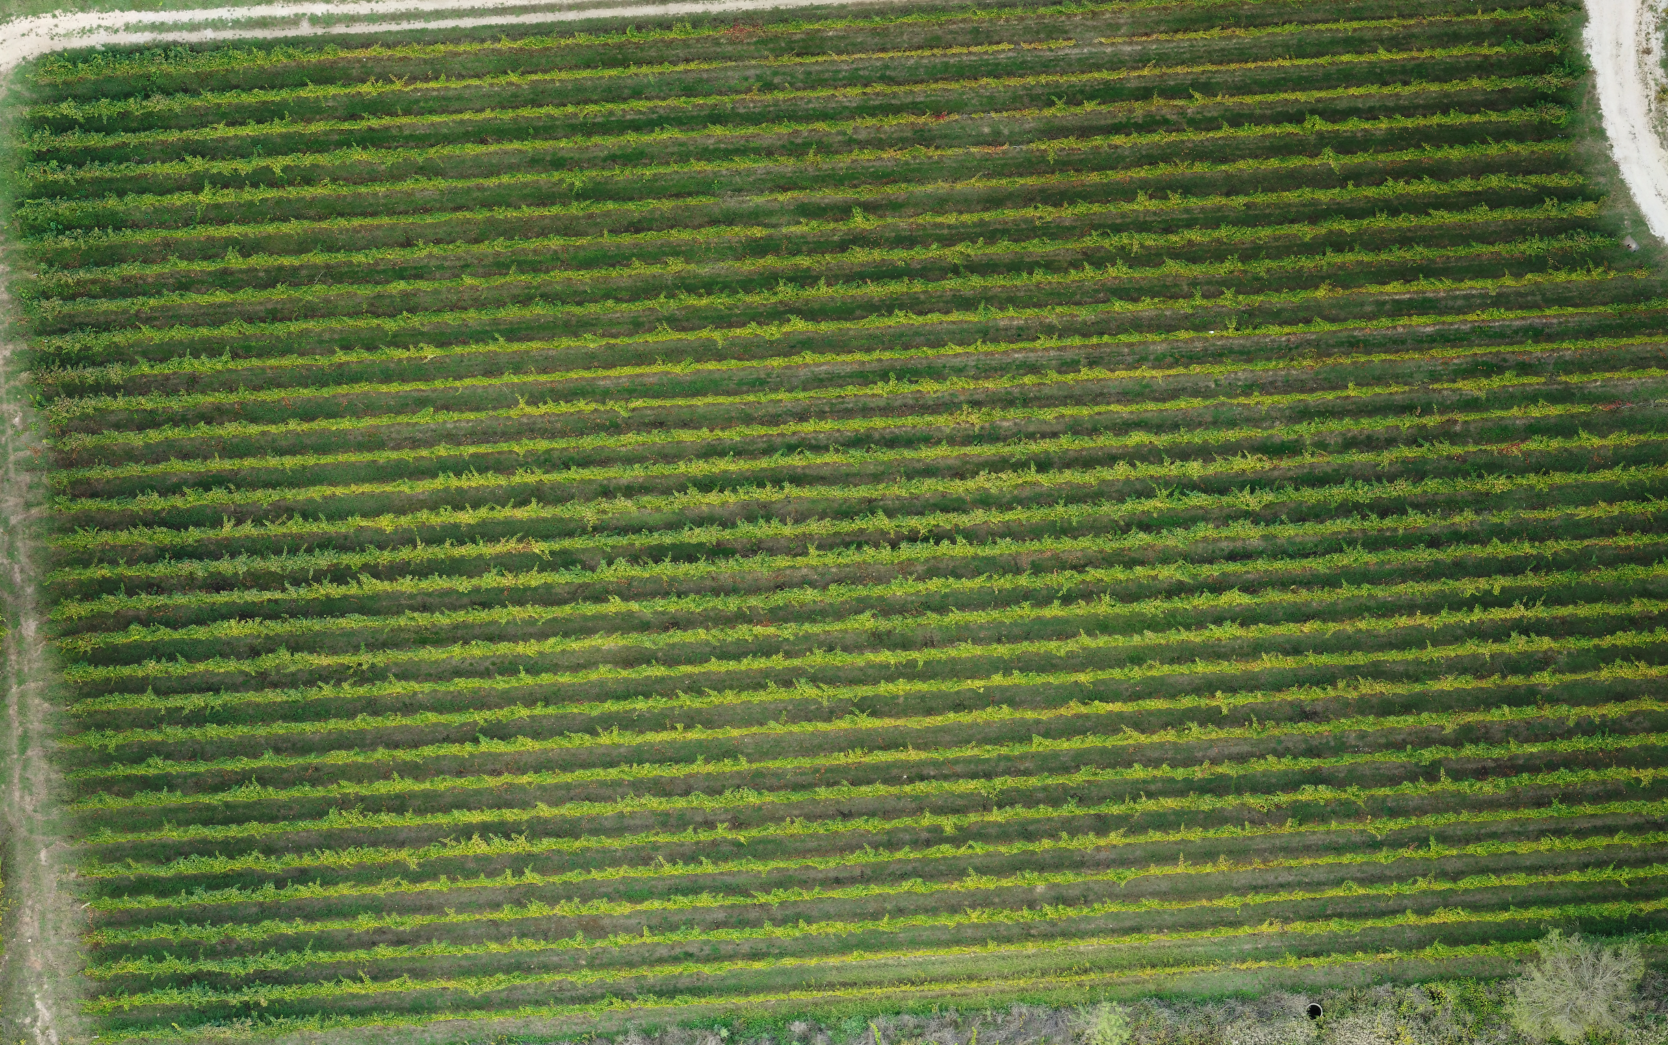
\includegraphics[width=\linewidth]{Aerial Image2.png}
		\caption{Aerial image sample used for waypoint detection
			\cite{b5}}
		\label{fig_Aerial}
	\end{figure}
	
	\subsubsection{Image Segmentation}\label{Image Segmentation}\leavevmode
	
	Image segmentation is this project's most computationally intensive section, and its outcome directly impacts the system's overall accuracy. Given the RGB sub-images, it is important to identify the exact locations where crops exist, which is done by processing the image and generating a binary mask. The following section introduces and implements two semantic segmentation methods, and their results are assessed.
	
	\paragraph{Color-Filtering Based Image Segmentation}\leavevmode
	
	The initial idea for image segmentation of crops in agricultural fields was to apply color filtering methods to isolate the areas having a green color. This method was first used by analyzing the image's green channel but performed poorly for a few reasons. First, the green channel filtering method cannot filter white pixels since they also include a large amount of green color. Second, there are sections of crops with color tending to yellow, which were unintentionally removed from the layer mask. The two issues mentioned were later resolved using a prefiltering for white pixels removal and also by converting the RGB image to HSV format (Hue, Saturation, and Value) so that it would be possible to filter the pixels based on their color considering their Vegetation Index (VI).
	
	Next, a K-means clustering method was applied to the color-based filtered image to highlight the areas, including crops. The clustering helped remove sparse pixels identified as crops and unite the areas where crops exist. The Parameters of the K-means algorithm were defined in an iterative approach to determine the best-performing setting,
	
	Without a high computational cost, this method can generate an accurate binary mask indicating the areas where vegetation exists. However, examining this method on the images taken from different fields with various crops, it was observed that it fails when unwanted vegetation like grass and weeds exists. Since the model filters the pixels based on their color, it cannot isolate crops without including the other vegetation. The same results in
	\cite{b5} are observed.
	Fig.
	\ref{fig2:kmeans} shows the performance of this method on different sub-images.
	
	
	\begin{figure}[t]
		\centering
		\includegraphics[width=\linewidth]{kmeans_predictions.png}
		\caption{Color-Filtering Based Image Segmentation
			\cite{b5}}
		\label{fig2:kmeans}
	\end{figure}
	
	
	\paragraph{Unet-Based Image Segmentation}\leavevmode
	
	The limited performance of color-based image segmentation in crop fields indicates the need for an intelligent model that can recognize the crops using more complicated methods. Utilizing machine learning methods to train semantic segmentation models has proven to be a reliable solution for crop detection. In this approach, a Unet network was chosen as the primary image segmentation tool (Fig.
	\ref{fig_Unet})
	and was trained on a dataset developed by
	\cite{b5}
	.This dataset consists of quadcopter-based aerial images taken from three vineyards with corresponding ground truth images, indicating the location of vines in the vineyard.
	
	The original and ground truth images were initially split into sub-images using a sliding window of size 512 by 512 pixels to use the annotated aerial images. The sliding step size was chosen to be 50 pixels, which resulted in more sample data for training. The resulting dataset consists of 5089 sub-images, which are divided into train, test, and validation sets with a ratio of 80\%\
	, 10\%\
	, 10\%\
	.
	
	The Unet model was trained in 50 epochs, which reached the early stopping condition at epoch 7 with an accuracy of 96\%\ and a loss value of 0.09. The predictions of this model on test data prove its ability to semantically segment crops in different conditions, even in the presence of unwanted vegetation (Fig. 
	\ref{fig2:Unet_Segmentation})
	
	
	\begin{figure}[t]
		\includegraphics[width=\linewidth]{UNET.png}
		\caption{Unet model architecture}
		\label{fig_Unet}
	\end{figure}
	
	\begin{figure}[t]
		\centering
		\includegraphics[width=\linewidth]{unet_predictions.png}
		\caption{Unet-Based Image Segmentation
			\cite{b5}}
		\label{fig2:Unet_Segmentation}
	\end{figure}
	
	\subsubsection{Crop Row Detection}\label{Crop Row Detection}\leavevmode
	
	The crop row detection process aims to assign a straight line with a defined slope and intercept each group of white pixels annotated as crops in the binary mask. This study analyzed and implemented two approaches—linear regression and the Hough Transform—for this purpose.
	
	\paragraph{Linear Regression}\label{Linear Regression}\leavevmode
	
	This experiment used the binary layer mask of segmented crops to assign each pixel to its corresponding crop row. The first step involved determining the optimal angle of the crop rows through an iterative algorithm, assuming that all rows are parallel and share the same slope. Once the slope was defined, the x and y coordinates of the white pixels were rotated to align the crop rows vertically, simplifying the clustering process.
	
	At this stage, the K-means algorithm was applied with a customized loss function designed to minimize the least square error of the distances between the white pixels and a vertical line. Unlike standard loss functions that measure the distance from a centroid point, this approach considered each cluster centered around a line, not a point.
	
	Given the variability in the number of clusters across different images, the clustering algorithm is initiated by grouping nearby pixels. When a pixel was too distant from the existing group, it was treated as the center of a new cluster. However, this approach led to the formation of numerous unwanted clusters. To address this, adjacent clusters were merged in a subsequent step. Finally, the initial rotation of the pixel coordinates was reversed to visualize the resulting clusters. As illustrated in the results, even after merging close clusters, the method failed to accurately identify crop rows, leading to complications in the later stages of the project. To conclude the experiment, linear regression was applied to fit a line to the pixels within each cluster. However, the results indicated that this clustering and linear regression approach is ineffective for defining crop rows, necessitating exploring alternative methods.
	
	\paragraph{Hough Transform}\label{Hough Transform}\leavevmode
	
	Another widely used solution for crop row detection is the Hough Transform. This computer vision technique is primarily designed to identify geometric shapes in images, making it particularly effective for detecting lines and curves. In this project, the Hough Transform was employed as an alternative to the linear regression model for predicting crop rows. Implementing this method requires significantly less preprocessing and image manipulation, mainly due to the availability of related packages in OpenCV. When the Hough Transform was applied to the images, multiple lines were detected for each crop row, as illustrated in Fig.
	\ref{fig_Hough_Init}. These lines successfully covered the crop rows, indicating the method's effectiveness in line detection. To refine the results and assign only one line per crop row, the detected lines were merged, and a single line was calculated using the average slope and intercept of the detected lines. The final results are presented in Fig.
	\ref{fig_Hough_mod}.
	
	\begin{figure}[t]
		\centering
		\begin{subfigure}{\linewidth}
			\centering
			\includegraphics[width=0.7\linewidth]{Hough initial2.png}
			\caption{Initial Hough transform implementation}
			\label{fig_Hough_Init}
		\end{subfigure}
		
		\vspace{0.5cm} % Adjust the space between the two subfigures as needed
		
		\begin{subfigure}{\linewidth}
			\centering
			\includegraphics[width=0.7\linewidth]{Hough Revised2.png}
			\caption{Modified Hough transform implementation}
			\label{fig_Hough_mod}
		\end{subfigure}
		
		\caption{Crop row detection methods using Hough transform \cite{b5}}
		\label{fig:comparison}
	\end{figure}
	
	
	\subsubsection{Path Waypoint Generation}\label{Path Waypoint Generation}\leavevmode
	
	As stated in previous steps, the most computational parts of this study are image segmentation and crop row detection. Determining crop rows as lines with defined slope and intercept makes calculating a line indicating the path straightforward. The path is defined as a line parallel to two neighboring crop rows at an equal distance from each other.
	Waypoints can be defined by choosing a specific number of equally spaced points along each path. The local coordination of these waypoints is stored for later study steps.
	
	\subsubsection{Reconstruction of Aerial Image}\label{Reconstruction of Aerial Image}\leavevmode
	
	Following the image splitting described in the section
	\ref{Preprocessing}, the image processing tasks outlined earlier will be applied to each segment of the leading aerial image. The goal is to determine and record the waypoint coordinates within each segment. Once the waypoint coordinates are computed, the initial image must be reconstructed and assembled. Subsequently, the waypoint coordinates need to be converted to align with the coordinates of the newly assembled image.
	
	\subsection{Waypoint Generation}\label{Waypoint Generation}
	To obtain the corresponding global coordinates of the points identified in the images, an analytical approach and mathematical algorithm are required. This process involves using the global coordinates of the camera at the time of image capture, along with the camera's height. The conversion process is divided into two phases: first, converting pixel coordinates into meter units, and second, converting these meter distances into the global coordinate system.
	
	\begin{figure}[t]
		\centering
		\includegraphics[width=0.7\linewidth]{waypoint_geometry}
		\caption{Geometrical representation of waypoint generation}
		\label{fig:waypointgeometry}
	\end{figure}
	
	
	\subsubsection{Pixel to Meter Conversion}\label{Pixel to Meter Conversion}\leavevmode
	
	Assuming the camera is positioned at the center of the image at a height of \( h \), and given the angle \( \theta \) (See Fig. \ref{fig:waypointgeometry}), the conversion of pixel position to distance is described by the following equations:
	\begin{equation}
		\tan \theta = \frac{x}{h} \implies x = \tan \theta  \cdot h
		\label{eq:1}
	\end{equation}
	
	Where \( x \) is the distance from the camera position to the image's edge in meters.
	
	Assuming the image to be in a square frame and the resolution is \( L \) by \( L \) pixels, then:
	
	\begin{equation}
		{x}=\frac{L}{2}\left(pixel\right)
		\label{eq:2}
	\end{equation}
	
	using equations (\ref{eq:1}) and (\ref{eq:2}) implies:
	
	\begin{equation}
		1 \text{ (pixel)} = 2h \cdot \frac{\tan \theta}{L} \text{ (m)}
		\label{eq:3}
	\end{equation}
	
	
	Achieving equation (\ref{eq:3}), the actual distance between the position of the quadcopter and any point on the ground corresponding to coordination \((x, y)\) in the image can be calculated. 
	
	To generate the waypoints, which are in the form of latitude and longitude, a conversion factor of meter to global coordination is required, which is shown in equation (\ref{eq:4}) 
	
	\begin{equation}
		1 \text{ (m)} = 0.00001^\circ
		\label{eq:4}
	\end{equation}
	
	Thus, using equations (\ref{eq:3}) and (\ref{eq:4}) implies the final conversion factor for calculation of the change in global coordination as defined in equation (\ref{eq:5}):
	
	\begin{equation}
		1 \text{ (pixel)} = 0.00002 \times h \cdot \frac{\tan \theta}{L}^\circ
		\label{eq:5}
	\end{equation}
	
	Lastly, the relative change in global coordinates is added to the quadcopter's GPS-derived coordinates along the latitude and longitude axes to generate waypoints and obtain accurate global pixel coordinates.
	
	\section{Experimental Setup}\label{Experimental Setup}
	In alignment with the primary objective of this research, which aimed to develop an integrated system for acquiring live aerial imagery and calculating global coordinates for path waypoints, an experimental setup incorporating a camera and radio transmission system was designed and implemented. Using the RC805 radio transmission system, a wireless connection between the camera and a computer was established to facilitate the transfer of live images captured by a GoPro Hero4 camera. The experimental configuration is illustrated in Fig.
	\ref{EXP}.
	
	The previously described image processing features were consolidated into a program with a graphical user interface (GUI). This system allows for two modes of operation: offline, where pre-existing images stored locally on the computer are loaded, and online, where live-stream imagery from the camera is received. The results of each image processing step are subsequently displayed in the program's output, providing a visual representation of the logic underpinning the generated waypoints.
	
	
	
	
	\begin{figure}[t]
		\includegraphics[width=\linewidth]{Setup of experiment.png}
		\caption{Experimental setup of proposed waypoint generation system}
		\label{EXP}
	\end{figure}
	
	\section{Results and Discussion}\label{Results and Discussion}
	
	
	
	
	\section{Conclusion}\label{Conclusion}
	The paper addresses the growing need for precise navigation systems utilized by autonomous agricultural mobile robots. It presents a hardware setup and an image processing procedure for acquiring live aerial images of agricultural fields and identifying the global coordinates of the waypoints placed within the field. These coordinates serve as reference points for mobile robot navigation systems. The environmental information of the field is gathered using high-resolution RGB aerial images acquired by cameras mounted on quadcopters, along with the global coordinates of the quadcopter acquired by GPS modules. A radio transmission system transfers data from the quadcopter position to the processing unit. The procedure for extracting the global coordinates of the path from the acquired aerial images is defined as an image processing algorithm encompassing image segmentation, crop row detection, and waypoint generation.
	
	Initially, the aerial image is divided into equal-sized sub-images to ensure uniform inputs for the image processing algorithms. Two image segmentation methods, namely color-filtering-based and Unet-based, are considered to identify the position of the crops in the resulting sub-images. The study demonstrates that while both methods can perform image segmentation tasks, the color filtering approach is ineffective in fields with other unwanted vegetation, such as grass and weeds. Conversely, the trained Unet model achieves an accuracy of 96\%\ and generates satisfactory predictions of plant positions in different fields. Consequently, the Unet-based method is selected as the primary image segmentation tool.
	
	Following the segmentation step, linear regression and Hough Transform methods are evaluated for crop row detection. The analysis reveals that the linear regression method's complexity, encompassing pixel clustering and line fitting, renders it a cumbersome solution for this task, leading to unsatisfactory crop row detections. In contrast, implementing Hough Transform as an alternative crop row detection approach results in more accurate estimated lines. Waypoints are defined as equally spaced points on the path, calculated as parallel lines between two crop rows.
	
	The global coordinates of the defined waypoints are obtained through the reconstruction and mapping of the local coordinates found in each sub-image to the local coordinates of the original image. Subsequently, the global coordinates are calculated based on the local position of pixels and the global coordinates of the camera at the time of image capture and stored for further utilization.
	
	
	\begin{thebibliography}{00}
		\bibitem{b1} Y. Yang et al., "Real-time detection of crop rows in maize fields based on autonomous extraction of ROI," Expert Systems with Applications, vol. 213, p. 118826, 2023.
		\bibitem{b2} J. Shi, Y. Bai, Z. Diao, J. Zhou, X. Yao, and B. Zhang, "Row detection BASED navigation and guidance for agricultural robots and autonomous vehicles in row-crop fields: methods and applications," Agronomy, vol. 13, no. 7, p. 1780, 2023.
		\bibitem{b3} V. R. Ponnambalam, M. Bakken, R. J. Moore, J. Glenn Omholt Gjevestad, and P. Johan From, "Autonomous crop row guidance using adaptive multi-roi in strawberry fields," Sensors, vol. 20, no. 18, p. 5249, 2020.
		\bibitem{b4} N. Cunha, T. Barros, M. Reis, T. Marta, C. Premebida, and U. J. Nunes, "Multispectral image segmentation in agriculture: A comprehensive study on fusion approaches," in Iberian Robotics conference, 2023: Springer, pp. 311-323.
		\bibitem{b5} T. Barros et al., "Multispectral vineyard segmentation: A deep learning comparison study," Computers and electronics in agriculture, vol. 195, p. 106782, 2022.
		\bibitem{b6} G. Ronchetti, A. Mayer, A. Facchi, B. Ortuani, and G. Sona, "Crop row detection through UAV surveys to optimize on-farm irrigation management," Remote Sensing, vol. 12, no. 12, p. 1967, 2020.
		\bibitem{b7} M. Hassanein, M. Khedr, and N. El-Sheimy, "Crop row detection procedure using low-cost UAV imagery system," The International Archives of the Photogrammetry, Remote Sensing and Spatial Information Sciences, vol. 42, pp. 349-356, 2019.
		\bibitem{b8} M. D. Bah, A. Hafiane, and R. Canals, "CRowNet: Deep network for crop row detection in UAV images," IEEE Access, vol. 8, pp. 5189-5200, 2019.
		\bibitem{b9} I. Sa et al., "WeedMap: A large-scale semantic weed mapping framework using aerial multispectral imaging and deep neural network for precision farming," Remote Sensing, vol. 10, no. 9, p. 1423, 2018.
		\bibitem{b10} S. Sankaran et al., "Low-altitude, high-resolution aerial imaging systems for row and field crop phenotyping: A review," European Journal of Agronomy, vol. 70, pp. 112-123, 2015.
		\bibitem{b11} L. Comba, P. Gay, J. Primicerio, and D. R. Aimonino, "Vineyard detection from unmanned aerial systems images," Computers and Electronics in Agriculture, vol. 114, pp. 78-87, 2015.
		\bibitem{b12} K. Ramesh, N. Chandrika, S. Omkar, M. Meenavathi, and V. Rekha, "Detection of rows in agricultural crop images acquired by remote sensing from a UAV," International Journal of Image, Graphics and Signal Processing, vol. 8, no. 11, p. 25, 2016.
		\bibitem{b13} M. Pérez-Ortiz, J. Peña, P. A. Gutiérrez, J. Torres-Sánchez, C. Hervás-Martínez, and F. López-Granados, "A semi-supervised system for weed mapping in sunflower crops using unmanned aerial vehicles and a crop row detection method," Applied Soft Computing, vol. 37, pp. 533-544, 2015.
		\bibitem{b14} Y. Pang et al., "Improved crop row detection with deep neural network for early-season maize stand count in UAV imagery," Computers and Electronics in Agriculture, vol. 178, p. 105766, 2020.
		\bibitem{b15} N. Samet, S. Hicsonmez, and E. Akbas, "Houghnet: Integrating near and long-range evidence for bottom-up object detection," in Computer Vision–ECCV 2020: 16th European Conference, Glasgow, UK, August 23–28, 2020, Proceedings, Part XXV 16, 2020: Springer, pp. 406-423.
		\bibitem{b16} F.-A. Moreno, J. Monroy, J.-R. Ruiz-Sarmiento, C. Galindo, and J. Gonzalez-Jimenez, "Automatic waypoint generation to improve robot navigation through narrow spaces," Sensors, vol. 20, no. 1, p. 240, 2019.
	\end{thebibliography}
	
	\vspace{12pt}
	
	
\end{document}
